%%%%%%%%%%%%%%%%%%%%%%%%%%%%%%%%%%%%%%%%%
% Proceedings of the National Academy of Sciences (PNAS)
% LaTeX Template
% Version 1.0 (19/5/13)
%
% This template has been downloaded from:
% http://www.LaTeXTemplates.com
%
% Original author:
% The PNAStwo class was created and is owned by PNAS:
% http://www.pnas.org/site/authors/LaTex.xhtml
% This template has been modified from the blank PNAS template to include
% examples of how to insert content and drastically change commenting. The
% structural integrity is maintained as in the original blank template.
%
% Original header:
%% PNAStmpl.tex
%% Template file to use for PNAS articles prepared in LaTeX
%% Version: Apr 14, 2008
%
%%%%%%%%%%%%%%%%%%%%%%%%%%%%%%%%%%%%%%%%%

%----------------------------------------------------------------------------------------
%	PACKAGES AND OTHER DOCUMENT CONFIGURATIONS
%----------------------------------------------------------------------------------------

%------------------------------------------------
% BASIC CLASS FILE
%------------------------------------------------

%% PNAStwo for two column articles is called by default.
%% Uncomment PNASone for single column articles. One column class
%% and style files are available upon request from pnas@nas.edu.

\documentclass[a4paper]{article}
%\documentclass{pnastwo}

%------------------------------------------------
% POSITION OF TEXT
%------------------------------------------------

%% Changing position of text on physical page:
%% Since not all printers position
%% the printed page in the same place on the physical page,
%% you can change the position yourself here, if you need to:

% \advance\voffset -.5in % Minus dimension will raise the printed page on the 
                         %  physical page; positive dimension will lower it.

%% You may set the dimension to the size that you need.

%------------------------------------------------
% GRAPHICS STYLE FILE
%------------------------------------------------

%% Requires graphics style file (graphicx.sty), used for inserting
%% .eps/image files into LaTeX articles.
%% Note that inclusion of .eps files is for your reference only;
%% when submitting to PNAS please submit figures separately.

%% Type into the square brackets the name of the driver program 
%% that you are using. If you don't know, try dvips, which is the
%% most common PC driver, or textures for the Mac. These are the options:

% [dvips], [xdvi], [dvipdf], [dvipdfm], [dvipdfmx], [pdftex], [dvipsone],
% [dviwindo], [emtex], [dviwin], [pctexps], [pctexwin], [pctexhp], [pctex32],
% [truetex], [tcidvi], [vtex], [oztex], [textures], [xetex]

\usepackage{graphicx}
\usepackage{algorithmic}
\usepackage{algorithm2e}


%------------------------------------------------
% ADDITIONAL OPTIONAL STYLE FILES
%------------------------------------------------

%% The AMS math files are commonly used to gain access to useful features
%% like extended math fonts and math commands.

\usepackage{amssymb,amsfonts,amsmath}

%------------------------------------------------
% OPTIONAL MACRO FILES
%------------------------------------------------

%% Insert self-defined macros here.
%% \newcommand definitions are recommended; \def definitions are supported

%\newcommand{\mfrac}[2]{\frac{\displaystyle #1}{\displaystyle #2}}
%\def\s{\sigma}


\begin{document}

%----------------------------------------------------------------------------------------
%	TITLE AND AUTHORS
%----------------------------------------------------------------------------------------

\title{Report on Machine Learning Lab, Ex 3} % For titles, only capitalize the first letter


\author{Mostafa Mohamed, Omar Kassem}%\affil{1}{Alberts-Ludwig Universt\"at Freiburg}}
%James Smith\affil{2}{University of Oregon}
%\and
%Jane Smith\affil{1}{}}

%\contributor{Submitted to Proceedings of the National Academy of Sciences of the United States of America}

%----------------------------------------------------------------------------------------

\maketitle % The \maketitle command is necessary to build the title page

%\begin{article}

%----------------------------------------------------------------------------------------
%	ABSTRACT, KEYWORDS AND ABBREVIATIONS
%----------------------------------------------------------------------------------------

%\begin{abstract}
%Abstract
%\end{abstract}

\section{Introduction}
This is a report about the deep learning lab, exercise 3. The general task of this assignment was to use Tensorflow/keras to implement a convolutional neural network to train it on solving a search problem and compare it to the A* search algorithm. As well as trying different configurations and architectures of the neural networks.

\section{Search problem}
The given problem was find a target position in a given maze. We were given a simulator that can visualize our algorithm or the given reference A* algorithm. 

\section{Architecture}
\begin{itemize}
\item Input: There was a given script that generates the train/validation data according to the A* algorithm. It starts from a variety of random positions and tries to search for the target. The A* reaches the target optimally.

\item Network: We used Keras to implement our neural network. We implemented a network that consists of 2 fully-connected layers followed by 3 convolutional layers. We tried different activation functions on some layers (like tanh), mostly the relu showed the best results.
\end{itemize}

\section{Results}
We tried different configurations for the running.
\begin{itemize}
\item Smaller local view: This possibility lead for an accuracy of ~80\%
\item Different history length: 
	\begin{itemize}
		\item 10: 15/20 tests lead to 100\% accuracy, 4/20 to 96\% and 1/20 to 92\% accuracies respectively.
		\item 6: 19/20 tests lead to 100\% accuracy and 1/20 to 96\%.
		\item 4: 15/20 tests lead to 100\% accuracy and 5/20 to 96\%.
	\end{itemize}
\item Changing the target after training: Lead to accuracy ~45\%, there was an interesting observation in this case, that the agent was smart enough to learn from it's own mistakes; in the sense that after it goes in a dead end path, it can go back and try different paths. Sometimes there was enough steps remaining to achieve the goal, sometimes not.
\item Changing the map after training: lead to 0\% accuracy, it got stuck in a lot of parts of the map because it was so unfamiliar.


\end{itemize}

\section{Improvements}
To improve the results we can try to train with different strategies.
\begin{itemize}
\item Train the agent on a several target locations, with a slightly longer history and/or larger view. We believe that this will improve the results on a given map, because the agent will get a better grasp of how the map looks like generally and how deadends look like also, and won't be fixed on a specific target point. However this will need much more training, because the agent can get confused easily if it was trained poorly on different targets, because the target's area isn't that relevant that much since it can change usually.

\item We can have a slightly different strategy for storing history that can for example store the locations visited previously so it will learn the nogood areas (then we just store the nogood areas), while finding the target, hence accumulating failing experience, and try not to repeat bad areas to reach the target. This should show a potential improvement.

\end{itemize}

%----------------------------------------------------------------------------------------
%	FIGURES AND TABLES
%----------------------------------------------------------------------------------------

%% Adding Figure and Table References
%% Be sure to add figures and tables after \end{article}
%% and before \end{document}

%% For figures, put the caption below the illustration.
%%
%% \begin{figure}
%% \caption{Almost Sharp Front}\label{afoto}
%% \end{figure}
\iffalse
\begin{figure}[h]
\centerline{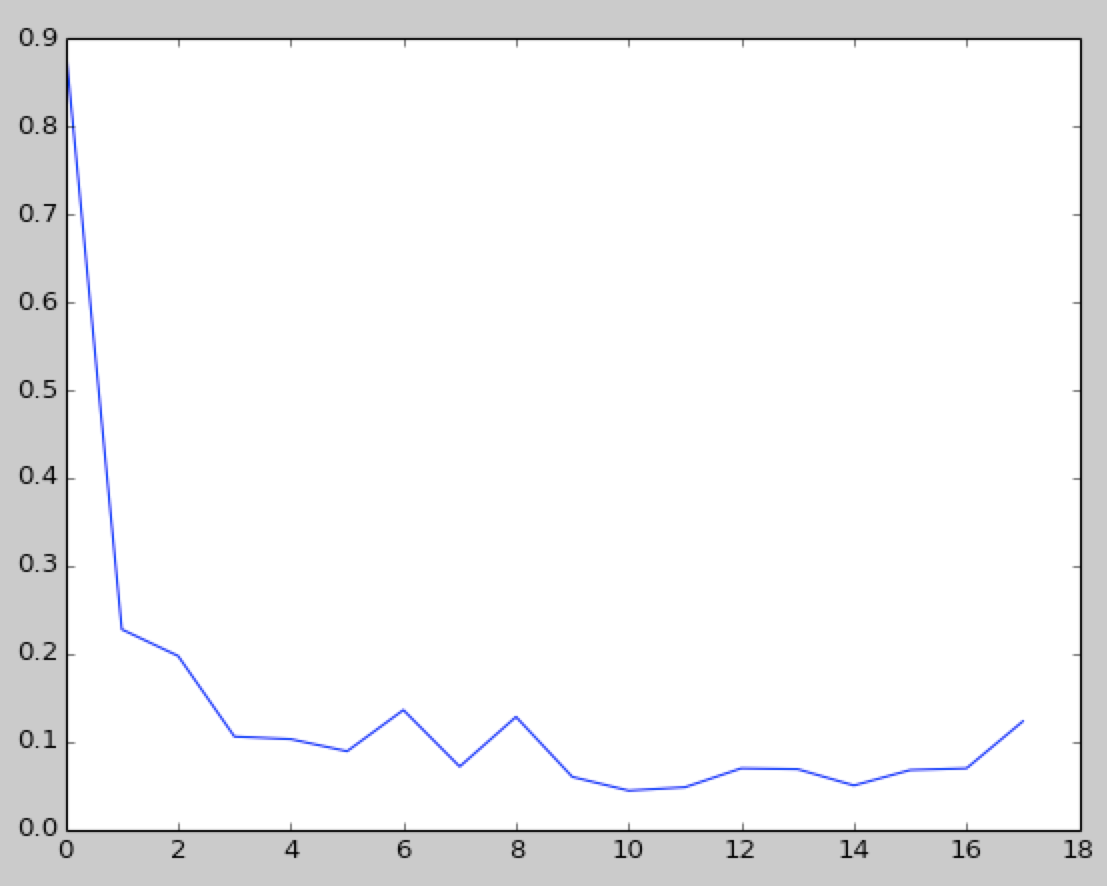
\includegraphics[width=0.4\linewidth]{2L3C.png}}
\caption{2 Layers, 3 Channels, Accuracy: 89\%}\label{placeholder}
\end{figure}

\begin{figure}[h]
\centerline{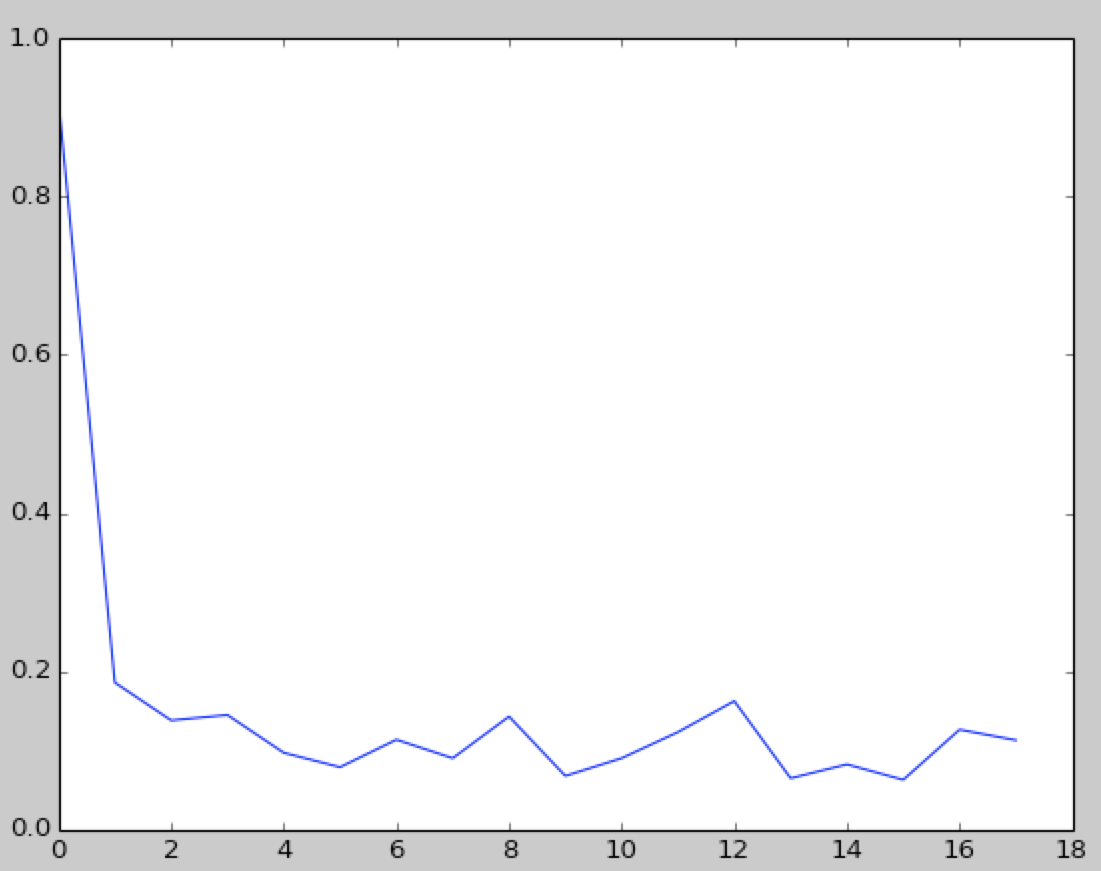
\includegraphics[width=0.4\linewidth]{2L4C.png}}
\caption{2 Layers, 4 Channels, Accuracy: 91\%}\label{placeholder}
\end{figure}

\begin{figure}[h]
\centerline{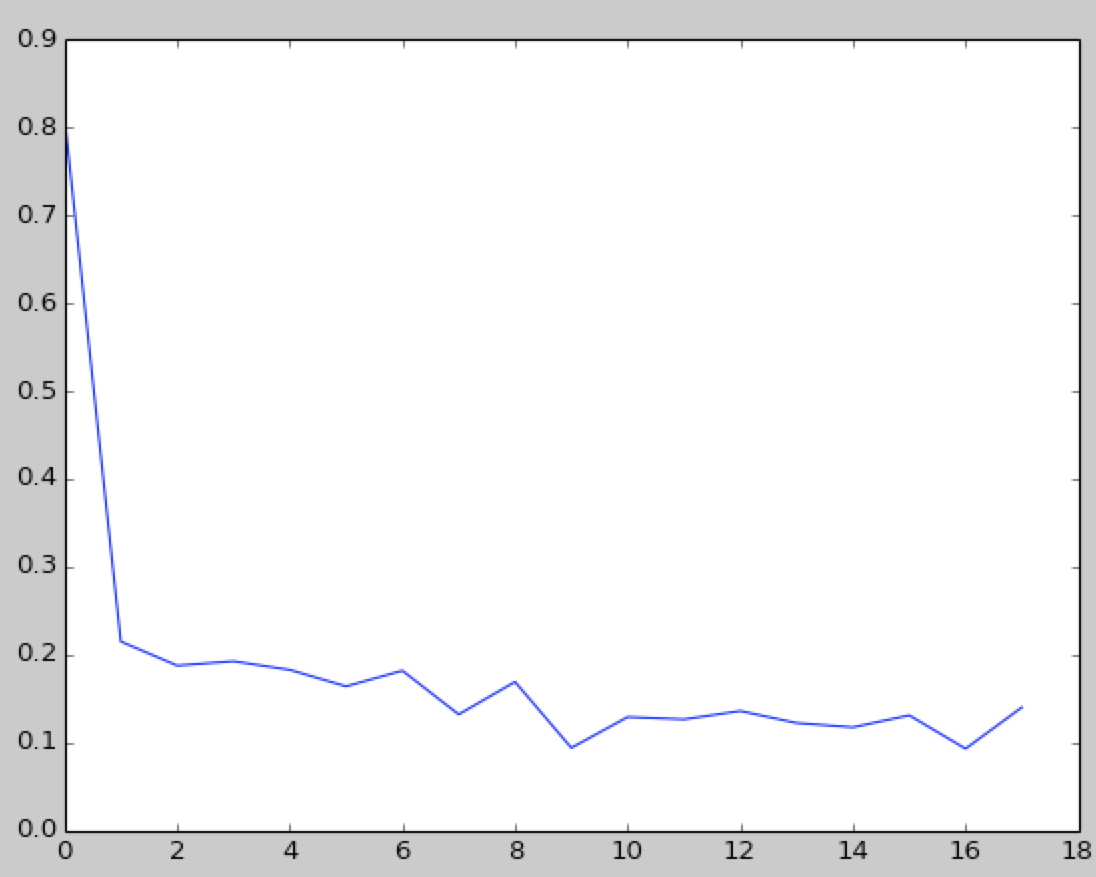
\includegraphics[width=0.4\linewidth]{3L3C.png}}
\caption{3 Layers, 3 Channels, Accuracy: 92\%}\label{placeholder}
\end{figure}

\begin{figure}[h]
\centerline{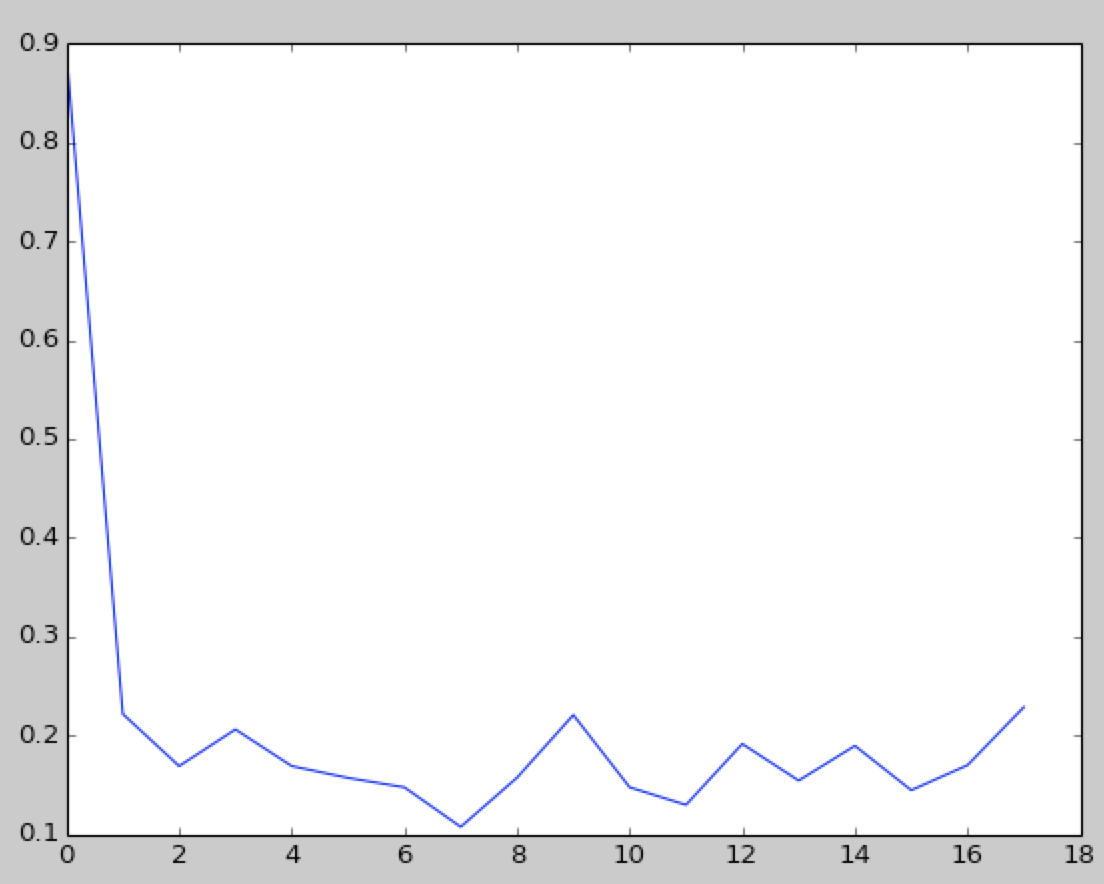
\includegraphics[width=0.4\linewidth]{3L4C.png}}
\caption{3 Layers, 4 Channels, 87\%}\label{placeholder}
\end{figure}
\fi
%% For Tables, put caption above table
%%
%% Table caption should start with a capital letter, continue with lower case
%% and not have a period at the end
%% Using @{\vrule height ?? depth ?? width0pt} in the tabular preamble will
%% keep that much space between every line in the table.

%% \begin{table}
%% \caption{Repeat length of longer allele by age of onset class}
%% \begin{tabular}{@{\vrule height 10.5pt depth4pt  width0pt}lrcccc}
%% table text
%% \end{tabular}
%% \end{table}

%% For two column figures and tables, use the following:

%% \begin{figure*}
%% \caption{Almost Sharp Front}\label{afoto}
%% \end{figure*}

%% \begin{table*}
%% \caption{Repeat length of longer allele by age of onset class}
%% \begin{tabular}{ccc}
%% table text
%% \end{tabular}
%% \end{table*}

%----------------------------------------------------------------------------------------

\end{document}
